%\documentclass[apjl]{emulateapj}

%\usepackage{amsmath}
%\usepackage{amssymb}
%\usepackage{color}
%\usepackage{natbib}

% Use only LaTeX2e, calling the article.cls class and 12-point type.

\documentclass[12pt]{article}

% Users of the {thebibliography} environment or BibTeX should use the
% scicite.sty package, downloadable from *Science* at
% http://www.sciencemag.org/authors/preparing-manuscripts-using-latex
% This package should properly format in-text
% reference calls and reference-list numbers.

\usepackage{scicite}

\usepackage{times}

\usepackage{graphicx}
\usepackage{hyperref}


% The preamble here sets up a lot of new/revised commands and
% environments.  It's annoying, but please do *not* try to strip these
% out into a separate .sty file (which could lead to the loss of some
% information when we convert the file to other formats).  Instead, keep
% them in the preamble of your main LaTeX source file.


% The following parameters seem to provide a reasonable page setup.

\topmargin 0.0cm
\oddsidemargin 0.2cm
\textwidth 16cm
\textheight 21cm
\footskip 1.0cm


%The next command sets up an environment for the abstract to your paper.

\newenvironment{sciabstract}{%
\begin{quote} \bf}
{\end{quote}}


\newcommand{\MSun}{M_\odot}
\newcommand{\RSun}{R_\odot}
\newcommand{\Rstar}{R_*}
\newcommand{\Mstar}{m_*}
\newcommand{\MBH}{M_\mathrm{BH}}

\def\aj{Astronomical Journal}                 % Astronomical Journal
\def\apj{Astrophysical Journal}                % Astrophysical Journal
\def\apjl{Astrophysical Journal}             % Astrophysical Journal, Letters
\def\pasj{PASJ}
\def\apjs{ApJS}              % Astrophysical Journal, Supplement
\def\mnras{MNRAS}            % Monthly Notices of the RAS
\def\prd{Phys.~Rev.~D}       % Physical Review D
\def\prl{Phys.~Rev.~Lett}    % Physical Review Letters
\def\cqg{Class.~Quant.~Grav.~}%Classical and Quantum Gravity
\def\araa{ARA\&A}             % Annual Review of Astron and Astrophys
\def\nat{Nature}              % Nature
\def\aap{A\&A}                % Astronomy and Astrophysics
\def\na{New Astronomy}

%\newcommand{\will}[1]{\textcolor{cyan}{#1}}
%\newcommand{\ilya}[1]{\textcolor{red}{#1}}

\newcommand{\onesigrange}[3]{\ensuremath{#1^{+#2}_{-#3}}}
\newcommand{\alpharangeone}{\onesigrange{2.05}{0.14}{0.13}}
\newcommand{\alpharangetwo}{\onesigrange{2.05}{0.14}{0.13}}
\newcommand{\alpharangethree}{\onesigrange{2.11}{0.19}{0.17}}
\newcommand{\alpharangefour}{\onesigrange{2.15}{0.13}{0.13}}

\title{Comment on ``An excess of massive stars in the local 30 Doradus starburst''}

\author{Will M. Farr,$^{1,2\ast}$ Ilya Mandel$^{1\ast}$\\
\normalsize{$^1$Institute of Gravitational Wave Astronomy and School of Physics and Astronomy,}\\
\normalsize{University of Birmingham, Birmingham, B15 2TT, United Kingdom}\\
\normalsize{$^2$Center for Computational Astrophysics, Flatiron Institute}\\
\normalsize{162 Fifth Avenue, New York NY 10010, United States} \\
\normalsize{$^\ast$E-mail: wmfarr@star.sr.bham.ac.uk, imandel@star.sr.bham.ac.uk}
}

\date{}

\begin{document}

% Double-space the manuscript.

\baselineskip24pt

% Make the title.

\maketitle



\begin{sciabstract}
%
%Schneider et al.~(Reports, 5 January 2018, p.~69) found more stars above 30 solar masses than predicted by a standard Salpeter initial mass function (IMF) in the 30 Doradus star-forming region.  They find an IMF power-law exponent of $1.90^{+0.37}_{-0.26}$ in contrast to the Salpeter exponent of $2.35$; however, the significant statistical uncertainty in their result is based on a flawed analysis of the data. Correcting this error we infer an exponent of $\alpharangeone$.  Although the mean of our posterior on the exponent suggests a steeper IMF, it is in fact more statistically significantly different (about 2-$\sigma$) from the Salpeter value.  We discuss the impact of assumptions regarding data set completeness and the star formation history model; alternative assumptions can shift the inferred exponent to $\alpharangethree$ and $\alpharangefour$, respectively.  We also consider an additional break in the IMF power law, but do not find convincing evidence for such a break.
%
Schneider et al.~(Reports, 5 January 2018, p.~69) used an ad hoc statistical method in their calculation of the stellar initial mass function. Adopting an improved approach, we reanalyse their data and determine a power law exponent of $\alpharangeone$. Alternative assumptions regarding data set completeness and the star formation history model can shift the inferred exponent to $\alpharangethree$ and $\alpharangefour$, respectively.
%Although our mean value is higher than Schneider et al's, it is more significantly different from the standard Salpeter value of 2.35.
\end{sciabstract}


%The universality of the initial mass function of stars is a hot topic in modern astrophysics, with impact on galactic evolution, supernovae, and gravitational-wave sources \cite{Kroupa:2002,Bastian:2010,deMinkBelczynski:2015}.
Schneider et al.\cite{Schneider:2018} use spectroscopic observations of young massive stars in
the 30 Doradus region of the Large Magellanic Cloud to infer a
shallower-than-expected stellar initial mass function (IMF).  They estimate the ages and masses of individual
stars with the BONNSAI Bayesian code \cite{Schneider:2017}, then obtain
an overall mass distribution by effectively adding together the posterior
probability density functions of individual stars.  There is no statistical
meaning to a distribution obtained in this way, which does not represent the
posterior probability density function on the mass distribution.

%Their conclusion is due to a faulty statistical methodology and several questionable assumptions which we discuss below.

%\citet{Schneider:2018} estimate the ages and masses of individual stars with the BONNSAI Bayesian code \citep{Schneider:2017}.  They then obtain an overall mass distribution by effectively adding together the posterior probability density functions of individual stars.  There is no statistical meaning to a distribution obtained in this way, and it does not represent the posterior probability density function on the underlying mass distribution.  %In fact, when the underlying distribution is a steeply decaying power law, as considered here, the approach of \citet{Schneider:2018} will yield a distribution biased toward the high-mass end.  The measurement uncertainty will ``smear out'' the masses of both low-mass and high-mass stars, but because there are far more low-mass stars than high-mass ones, this appears to yield more mass at the high end of the distribution, leading to a false conclusion of a shallower distribution.

Hierarchical Bayesian inference provides the statistically justified solution to
this problem \cite{Hogg:2010}.  Mandel\cite{Mandel:2010stat} specifically considered
inference on a mass distribution given a sample of uncertain measurements, and
we use a similar methodology here.  We interpret the Schneider et al.\cite{Schneider:2018}
inference on individual masses and ages as independent Gaussian likelihoods for
the logarithm of the mass and the age, with parameters fixed by matching the mean
parameter to the peak and the standard deviation parameter to the 68\% width of
the individual stellar distributions in the Schneider et al.\cite{Schneider:2018} data.
%We have performed fits similar to those described here using a heavier-tailed, Student T likelihood with few degrees of freedom and find equivalent results, suggesting that heavy tails in the likelihood are not particularly influential in this analysis.

For our fiducial analysis we model the star formation history as a truncated Gaussian distribution, and
generally find similar star formation history to Schneider et al.\cite{Schneider:2018}, with
the star formation rate in 30 Dor peaking about 4 Myr ago.  We impose broad priors
on the power--law exponent and the mean and standard deviation of the star
formation Gaussian.    We use the Hamiltonian Monte Carlo sampler Stan
\cite{STAN} to efficiently address the high-dimensional hierarchical problem
with free parameters for each star's actual mass and birth age in addition to
the IMF exponent and the mean and standard deviation of the star formation
history.

Figure \ref{fig:IMF} shows the inferred power-law exponent of the IMF.   We use the Schneider et al.\cite{Schneider:2018} fit to stellar lifetimes and assume
that their data set is complete above 15 solar masses (i.e.\ selecting only
those stars whose observed mass is above $15 \, M_\odot$
\cite{Loredo:2004,BBH:O1}).  We find
an exponent of $\alpha=\alpharangeone$ where the quoted value corresponds to the median
of the posterior distribution and the range to the 16th and 84th percentiles
(i.e.\ the symmetric 68\% credible interval).  %Correcting the erroneous
%statistical procedure used by Schneider et al.\cite{Schneider:2018}
Hierarchical Bayesian modelling steepens the preferred IMF
slope; our median $\alpha$ value lies about $1\, \sigma$ above the preferred value from
Schneider et al.\cite{Schneider:2018}.  More significantly, it narrows the uncertainty interval by more than a factor of 2.

The analysis above used the same assumptions as Schneider et al.\cite{Schneider:2018}.  Below, we consider the impact of three additional  assumptions: the stellar lifetime fit; the choice of the completeness limit; and the model for the star formation history.

%The fit to stellar lifetimes used by \citet{Schneider:2018} continues to decrease at high masses, in contrast to the expectation that stellar lifetimes should asymptote to a fixed minimum duration for high-mass stars set by the ratio of the energy to be released through nuclear fusion to the Eddington luminosity.
We perform an independent fit to the main sequence lifetimes
$\tau_{MS}$ of non-rotating massive stars of mass $M$ as modelled by Brott et al.\cite{Brott:2011} and K\"{o}hler et al.\cite{Kohler:2015}:
%
\begin{equation}
\ln \frac{\tau_{MS} (M)}{\textrm{Myr}} = 9.1973 - 3.8955 \ln\frac{M}{M_\odot} %\nonumber\\ &&
+ 0.6107 \left(\ln\frac{M}{M_\odot} \right)^2 - 0.0332 \left(\ln\frac{M}{M_\odot}\right)^3.
\end{equation}
%Our fit predicts longer lifetimes for stars more massive than $\sim 100 M_\odot$ than the \citet{Schneider:2018} fit.  Using our fit rather than the \citet{Schneider:2018} fit therefore leads to a steeper power-law exponent, $\alpharangetwo$, as there are fewer massive stars that should have already collapsed into invisible remnants in our model.
Following Schneider et al.\cite{Schneider:2018}, we increase the ``observable''
lifetime of a star by 10\% beyond its main sequence lifetime to account for
helium burning.  We find that this alternative fit does not impact the inferred IMF, yielding the same power-law exponent $\alpha=\alpharangetwo$.

The inferred power-law exponent is somewhat sensitive to
the choice of the cutoff mass for survey completeness.  The data of Schneider et al.\cite{Schneider:2018} show a relative scarcity of stars between 15 and 20 solar masses; changing the mass cutoff from $15 M_\odot$ to $20 M_\odot$ further steepens the inferred exponent to $\alpha=\alpharangethree$.    However, these fluctuations are within the expected statistical variation based on the sample size, as confirmed with posterior predictive
checking.  In particular, we there is no statistical evidence against the claim of Schneider et al.\cite{Schneider:2018} that
the survey is complete for $M \geq 15 \, \MSun$.

Finally, we consider an alternative star formation history model: a double exponential, with three free parameters: the time of the peak of the star formation rate and the (possibly different) decay constants before and after the peak.  This model allows for a sharper peak and longer tails than a Gaussian.  This star formation rate history model is consistent with the data, as tested with posterior predictive checking (see below).  However, it yields a power-law exponent $\alpha=\alpharangefour$, almost  $1\, \sigma$ steeper than for our fiducial analysis.  This indicates that the inferred IMF is sensitive to the systematics of the assumed model.

\begin{figure}
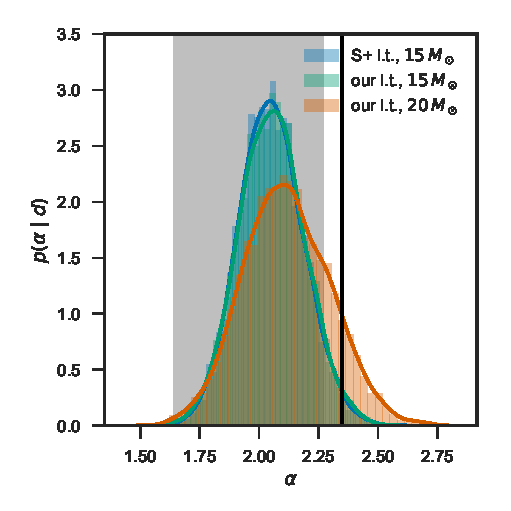
\includegraphics[width=\columnwidth]{alpha.pdf}
    		\caption{{\bf The posterior on the power-law exponent $\alpha$ is inferred from the observations $d$.}  See text for details on the four models (top to bottom in the legend): Schneider et al.\cite{Schneider:2018} stellar lifetimes, survey completeness for $M \geq 15 \, \MSun$, and Gaussian star formation history model (blue); as before, but with our lifetime fit (green); as before, but with completeness for $M \geq 20 \, \MSun$ (orange); as blue, but with a double-exponential star formation history model (pink).  The Salpeter power-law exponent is $-\alpha=-2.35$ \cite{Salpeter:1955}, indicated by a black line.  The 68.3\% range of power-law exponents derived by Schneider et al.\cite{Schneider:2018} is shaded in grey. }\label{fig:IMF}
\end{figure}

We also considered the possibility that the IMF power law has an additional break at higher masses, allowing for three free parameters: the mass at which the break happens and the exponent below and above the break.  However, we find that the data do not constrain the parameters of this more general model, and there is no statistical preference for a broken power-law model.

We confirm the stability of our conclusions with posterior predictive checking.
Figure \ref{fig:PPC} shows the distribution of observed masses and ages (i.e.,
the peak of the likelihood) from the Schneider et al.\cite{Schneider:2018} data overlain on the
range of mass and age distributions that would be observed from a large number
of data sets drawn according to our fitted IMF model.  The data are  consistent with our IMF model.  We have also confirmed that all of our models yield predictions for the numbers of stars heavier than $30 M_\odot$ and $60 M_\odot$ that are consistent with observations.

\begin{figure}
%\vspace{-1in}
    		    A.\\		\includegraphics[width=0.5\columnwidth]{dNdm-ppc-band.pdf}\\
               B.\\  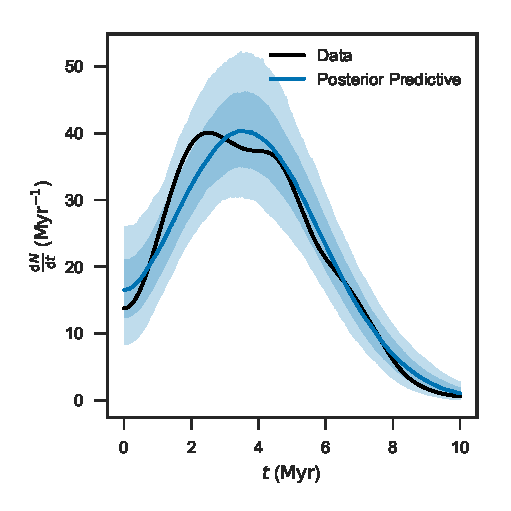
\includegraphics[width=0.5\columnwidth]{dNdt-ppc-band.pdf}
%\vspace{-1in}
    		\caption{{\bf Posterior predictive checking demonstrates that the observed data are consistent with being drawn from our model.} The observed distribution of (maximum likelihood) masses $M$ (A, black) and ages $t$ (B, black) and the range (median, 68\%, and 95\% credible intervals in blue) of distributions of mass and age from synthetic data drawn from our fitted model (i.e.\ the posterior predictive distribution).    %We see no evidence that our model is unable to account for the features in the observed data, including the apparent shallowing of the exponent of the mass distribution for $M \gtrsim 60 \, \MSun$.
		}\label{fig:PPC}
\end{figure}


We find that we can substantially reduce the statistical uncertainty in the IMF by applying an improved statistical analysis to the observations of young massive stars in 30 Doradus.  However, the systematics from modelling uncertainties, such as the assumed star formation history model, can potentially shift the inferred power-law exponent by more than the statistical uncertainty.   Furthermore, we adopted the mass and age posteriors for individual stars directly from Schneider et al.\cite{Schneider:2018}.  Imperfect stellar models or the inclusion of other complicating factors described by Schneider et al.\cite{Schneider:2018} (rotation, mass transfer, mergers, etc.) introduce further systematic uncertainty that could again shift the inferred IMF exponent.
%Although we do not discuss the possible systematic uncertainty on these due to imperfect stellar models or the inclusion of other complicating factors described by Schneider et al.\cite{Schneider:2018} (rotation, mass transfer, mergers, etc.), any systematics could again shift the inferred IMF exponent.
The combination of these factors makes it very challenging to infer the precise shape of the IMF even when a data set as good as that obtained by Schneider et al.\cite{Schneider:2018} is available.



{\bf Acknowledgments:} We are grateful to Schneider et al.\cite{Schneider:2018} for making the data on which their conclusions are based available for further study and analysis, and to Fabian Schneider personally for very useful discussions.  This analysis made use of \texttt{PyStan} \cite{STAN}, \texttt{astropy} \cite{astropy}, \texttt{numpy} \cite{numpy}, \texttt{scipy} \cite{scipy}, \texttt{matplotlib} \cite{matplotlib}, and \texttt{seaborn} \cite{seaborn} Python libraries.

{\bf Funding:} WMF and IM are partially supported by STFC.

{\bf Author contributions:} WMF and IM are jointly responsible for all aspects of this work.

{\bf Competing interests:} None.

{\bf Data and materials availability:} The code and \LaTeX source used to prepare this document are publicly available under an open-source MIT license at \url{https://github.com/farr/30DorIMF}.

%\section*{Acknowledgments}
%We are grateful to Schneider et al.\cite{Schneider:2018} for making the data on which their conclusions are based available for further study and analysis, and to Fabian Schneider personally for very useful discussions.  This analysis made use of \texttt{PySTAN} \cite{PySTAN}, \texttt{astropy} \cite{astropy}, \texttt{numpy} \cite{numpy}, \texttt{scipy} \cite{scipy}, \texttt{matplotlib} \cite{matplotlib}, and \texttt{seaborn} \cite{seaborn} Python libraries.  The code and \LaTeX source used to prepare this document are publicly available under an open-source MIT license at \url{https://github.com/farr/30DorIMF}.  WMF and IM are partially supported by STFC.

\bibliographystyle{Science}
\bibliography{Mandel}
\end{document}
